\documentclass[11pt]{article}
\usepackage[letterpaper, margin=0.75in]{geometry}
\usepackage{cite}
\usepackage{url}
\usepackage{multicol}
\usepackage{enumitem}
\usepackage{graphicx}
\usepackage{tabto}
\usepackage{float}
\setlength{\columnsep}{0.3in} 

\renewenvironment{abstract}
 {\small
  \begin{center}
  \bfseries \abstractname\vspace{-.5em}\vspace{0pt}
  \end{center}
  \list{}{%
    \setlength{\leftmargin}{0in}% <---------- CHANGE HERE
    \setlength{\rightmargin}{\leftmargin}%
  }%
  \item\relax}
 {\endlist}

\begin{document}
{
\vspace*{25px}
 \centering
 \LARGE Six Degrees of Collaboration \\ A Predator Pack's Guide to Success \\[1.5em]
 \large Sami Ghoche,
        George Lok,
        Devvret Rishi\\[1em]

        
	CS289 Final Project\\
	
	Harvard University
	
\vspace{75px}
}
\begin{multicols}{2}

\begin{abstract}

We introduce different collaboration policies for a pack of predators chasing a moving prey, ranging from complete collaboration to no collaboration at all. We operate in two settings: In the first setting, all predators can observe each other and their prey at all times, whereas in the second setting, predators can only observe what is directly in their line of sight. In the first setting, we present six collaboration policies that vary in efficiency both in terms of computational complexity and rate of success. In addition to evaluating the tradeoffs between these six mechanisms, we also present a successful trapping heuristic for a pack of coordinating predators. In the second setting, we present and compare two alternative search and destroy strategies through stigmergic communication. Our contributions will be useful for studies of predator/prey models in general, but may specifically be applicable in law enforcement settings involving a team of police officers chasing a fugitive from justice. 

\end{abstract}

\section{Introduction}
In nature, we observe that predator animals (including human beings) often collaborate when chasing a prey. This is because in some settings, a team of collaborating predators can achieve outcomes that separated individuals cannot, such as outcomes resulting from trapping behavior. However, collaboration nearly always exhibits large costs. First, collaborating agents have to split their rewards with their collaborators. In the animal world, this means gaining fewer resources; in law enforcement, this may mean receiving less credit for capturing criminals. Furthermore, collaboration always requires a form of coordination, and coordination is expensive. For example, we can consider ``perfect collaboration", whereby many predator agents act as a single unit that makes a single decision involving the movement of every agent in the team. This is essentially the same as having a centralized controller or a brain that directs each agent in the team. Such a centralized system though is not scalable, and there has been much research directed at developing scalable multi-agent systems in which computation is distributed among agents. 

In this paper, we assume that predators consider each other as collaborators instead of competitors, and they strive jointly to maximize an aggregate reward, meaning that all agents benefit equally when the prey is captured, regardless of which predator captured it. We also disregard the free-rider problem and assume that all predators actively make an effort to help the team instead of relying on other collaborators and reaping the benefits of the capture. For our experiments, we used the Berkeley Pacman framework \cite{Pacman}. because it allows for very general predator/prey model simulations. We operate in two settings: In the first setting, all predators can observe each other and their prey at all times, whereas in the second setting, predators can only observe what is directly in their line of sight. In the first setting, we present six different collaboration strategies with varying degrees of collaborative cost and efficiency: 1- Fully centralized collaboration. 2- Fully centralized collaboration of loosely coupled subteams. 3- Encrypted communication of actions between predators. 4- Communication of actions between predators that can be overheard by a prey. 5- Individual actions while taking into account positions of other predators. 6- No collaboration at all. The first five of these strategies require the notion of trapping behavior, and one of the main contributions of this paper is a successful heuristic that leads to trapping behavior. In the second setting, agents leave stigmergic trails behind them that decay with time, this is reminiscent of many examples of stigmergic communication observed in nature (for example in foraging ants \cite{beckers1992trails}). We compare two alternative strategies that predators can use to interact with the stigmergic trails that others leave behind. 1- Avoid these trails in an attempt to split up effectively and capture the prey. 2- Follow these trails in an attempt to congregate and corner the prey when it is found.\\
\indent The paper is organized into the following sections: Section 2 describes related work. Section 3 provides detailed descriptions with theoretical considerations of our six strategies in the first setting, and two strategies in the second setting. Section 4 describes our implementation using the Berkeley Pacman framework and the experiments we conducted. Section 5 presents our results and discusses them. Section 6 presents our conclusions and section 7 discusses future research directions. 

\section{Related Work}

Although there hasn’t been a significant amount of work explicitly exploring the tradeoffs between collaboration, communication and complexity in the settings that we chose to explore, our work was certainly motivated by a few different key papers we had read. 

In \textit{ Group Size, individual role differentiation and effectiveness of cooperation in a homogeneous group of hunters }, Escobedo et al. explore the emergence of cooperation in wolf-pack hunting using a very simple particle-based computational model \cite{escobedo2014group}. The setting that they were trying to model was similar to ours, as it involved multiple predatory agents collaborating together to try and capture a quarry and the authors were able to show that they could model the dynamics of how a wolf-pack goes about this task by modeling the interactions between wolves as each agent only trying to minimize their distance to the prey while maximizing its distance from the other wolves. Escobedo et al. showed that these simple interactions were able to explain much of the more complex collaborative behavior wolf-packs tended to demonstrate and this fact helped inform how we thought about trapping heuristics for our collaborative ghost agents, which we will cover later.

On a different side of our project, \textit{Reasoning About Joint Beliefs for Execution-Time Communication Decisions } by Roth et al. introduced us to the notion of thinking about the cost of communication in terms of run-time complexity and its relative benefit in the specific collaboration setting \cite{roth2005reasoning}. In their paper, the authors try to transform the typically highly intractable multi-agent POMDP into a more feasible problem by allowing communication when it’s believed to improve team performance. In doing so, they think explicitly about the cost and benefit of communication versus performance and also introduce us to a thinking about cost in terms of computational complexity, although in their case its more so to differentiate run-time versus plan-time costs.

As we have mentioned, we also explore a different setting where ghosts use stigmergic communication in order to disseminate information. The inspiration for this comes from \textit{Trails and U-turns in the Selection of a Path by the Ant Lasius niger} by Beckers et al  \cite{beckers1992trails}. In this paper, the authors discuss trail-laying algorithms employed by ant colonies that expedite foraging behaviors and explore tendencies of the ants to select certain paths, for example ones they had used previously. This inspired the section of our work where ghost agents lay trails of “pheromones” once they see Pacman, which can be thought of as a food source and we explore different manners by which other foragers could use these signals. 

The last paper we also felt was relevant to the discussion was \textit{ Collaborating and Learning Predators on a Pursuit Scenario } \cite{fredivianus2010collaborating}. Although this paper focused more on predator agents learning the best way to catch prey (either stationary or moving in their scenario) across only two scenarios, full centralization and full decentralization, we see strong similarities behind the motivation of both of our projects. As Fredivianus et al. also acknowledge in this paper, learning how to properly design these Multi-Agent Systems addresses some of the concerns over tradeoffs in distributed artificial intelligence and planning. 

 
\section{Description of Proposed Strategies}
\subsection{First Setting}
In the first setting, we propose six different strategies. Here they are in decreasing order of computational complexity:

\begin{enumerate}[leftmargin=0.25cm]
	\item Fully centralized collaboration
	
	In this strategy, we treat the predators as a single unit (called a team). Thus, a team's action is called a joint action. Joint action $\vec{a} = <a_1, a_2, ..., a_n>$, where $N$ is the number of predators. A centralized controller will evaluate every possible joint action, and select the joint action with the highest value. If there are at most $M$ possible actions a predator can take at any time step $t$, and a total of $T$ time-steps, the computational complexity of this strategy in every time-step will be $O(M^N)$ and thus, for the entire duration of the pursuit, the complexity would be $O(TM^N)$.
	
	\item Fully centralized collaboration of loosely coupled subteams
	
	In this strategy, we split the predators into $K$ subteams as evenly as possible. Each subteam $k$ will have a joint action $\vec{a_k}$. Joint action $\vec{a_k} = <a_1, a_2, ..., a_{\frac{N}{K}}>$. There is a centralized controller for each subteam that evaluates every possible joint action for that subteam and selects the one with the highest value. Since the computation for each subteam can be run in parallel, the complexity for this algorithm in one time-step will be $O(M^{\frac{N}{K}})$, and for the entire duration of the pursuit, the complexity would be $O(TM^{\frac{N}{K}})$. Therefore, this algorithm is asymptotically much faster than the first one, but its speed comes at a cost, since optimal joint actions for subteams might result in suboptimal joint actions for the larger team as a whole. 
	
	\item Encrypted communication of actions between predators.
	
	In this strategy, each predator decides which action to take on its own, but it takes into account the positions of other predators. This is important because predators will try to avoid each other in an attempt to minimize the area that the prey can maneuver in, effectively trapping it. However, since predators take individual decisions, they don't have a model of other predator's behaviors so they only take into account the current positions of other predators not where they are going to be in the next time step, which results in suboptimal decision-making based on inaccurate information. Communication can help with this problem: we can have predators take turns in deciding on an action and communicating it to all other predators once they have committed to it. So for example, predator 1 will decide on action $a_1$, and communicate it to predator 2, who will decide on $a_2$ based on the current positions of all other predators while taking into account predator 1's position AFTER taking action $a_1$. Predator 2 then communicates $a_2$ to predator 3, who decides on an action based on the positions of other predators and the positions that predators 1 and 2 will be in after taking actions $a_1$ and $a_2$ respectively, etc. until the last predator has a full picture of where all other predators will be and makes its decision based on those accurate future positions. Furthermore, we assume that communication is encrypted so the prey cannot overhear the communication and use it to its advantage. Each predator will look at the positions of each of the $N-1$ others and then evaluate each of the $M$ actions available to it. Since the predators have to wait for each other in turn, each time step will have a computational complexity of $O(N(N+M))$. Thus, the entire pursuit will have a complexity of $O(TN(N+M))$. This is exponentially faster than the first two algorithms, but the joint actions that this strategy yields in the end may be suboptimal. Additionally, there is a logistic cost to being able to communicate that we call $C$. This cost varies depending on the predator/prey domain. For example, in a law enforcement setting, this can be the cost of purchasing and maintaining walkie talkies. Since messages are securely encrypted in this strategy, there's another additional logistic cost that we call $S$. 
	
	\item Communication of actions between predators that can be overheard by the prey
	
	This strategy is very similar to the third one, except that at each step, the prey can overhear the entire communication between the predators because communication is not encrypted. This added information should allow the prey to take decisions faster (since it does not have to evaluate all possible actions of predators) and it will also reduce the uncertainty that the prey deals with and allow it to take decisions based on a more accurate belief model. As above, each time step will have a computational complexity of $O(N(N+M))$. Thus, the entire pursuit will have a complexity of $O(TN(N+M))$. Similarly, we still incur a logistic cost of $C$ because we are communicating, but there is no additional cost $S$ because the communication is no longer secure. 
	
	\item Individual actions while taking into account positions of other predators
	
	This strategy is similar to the previous two. However, there is no communication between predators here, so predators independently look at each other's current positions and take actions based on these current positions. Since predators no longer have to wait for each other in order to take decisions, the computation can be parallelized among the predators. So each time step will have a computational complexity of $O(N+M)$ and the entire pursuit will have a complexity of $O(T(N+M))$. This is linearly faster than the previous two algorithms and does not incur communication costs but actions are taken individually based on inaccurate information and are thus less optimal than in the previous two algorithms. 
	
	\item No collaboration at all
	
	In this strategy, predators do not collaborate or coordinate in any way. They simply each independently decide to chase the prey and take the action that minimizes their distance to the prey's current position. Assuming that distance evaluation takes constant time, we can parallelize the computation among the predators and conclude that the computational complexity of one time step is $O(M)$ and the computational complexity of the entire pursuit is $O(TM)$. It is important to note that while this strategy is by far the least complex, it does not inherently lead to any trapping behavior and essentially only allows for capturing the prey through accidental trapping (since we assume that the predators and the prey have the same speed and that the prey actively tries to evade predators).  
\end{enumerate}

\subsection{Second Setting}
In the second setting, we propose two different strategies revolving around the use of stigmergy.  In this setting, as ghosts do not know where Pacman is, they need a way to communicate with each other in order to find Pacman. The basic principle is that ghosts leave trails that other ghosts can sense when they are on top of them. The amount of trail left can depend on when ghosts see Pacman.  Ghosts will with high probability chase after Pacman if they see them.  Ghosts keep track of Pacman's last known position, and are biased to go towards that position if they don't see Pacman.  This last known position is reset if they arrive at the position and do not see Pacman.  Every time Pacman moves, the amount of trail decreases by a certain fraction.

\begin{enumerate}[leftmargin=0.25cm]
	\item Attractive Stigmergy
	
 	In attractive stigmergy, we adhere to the basic idea of stigmergy as presented by Beckers et. al \cite{beckers1992trails}. The idea is that ghosts will be able to follow trails in order to track down Pacman easier and then more easily capture Pacman as a group.  The basic mechanism is as follows: ghosts do not lay trails unless they either see Pacman or have an idea where Pacman is.  They lay more trail if they see Pacman than if they only have an idea where Pacman is.  Ghosts are more likely to choose a path that has more trail on it.  Finally, to prevent backtracking and to prevent them from sticking together, ghosts explicitly are less likely to take the reverse direction of the last action they do and are less likely to make an action that puts them on top of another ghost.
	
	\item Repulsive Stigmergy
	
	Taking advantage of the fact that we only need one ghost to capture Pacman, we reverse ghosts' reaction to trails and have them avoid paths that already have trail.  Ghosts always lay trail, but lay more trail if they think they know where Pacman is and significantly more trail if they directly see Pacman. Ghosts are more likely to choose a path that has less trail on it.  There's no need to prevent backtracking explicitly since the ghosts are unlikely to backtrack on their own trail.
\end{enumerate}


\section{Experimental Setup}
\subsection{General}
We simulated our approaches for both settings on the Berkeley Pacman game platform because it lent itself well to the general pattern of predator/prey models and was flexible enough to allow all the behavior that we wanted to simulate. In the Pacman game, the prey is a Pacman agent, and the predators are one or many ghosts. In the original game, Pacman moves around a map collecting food, and he wins once all the food on the map has been collected. He loses when a ghost catches him. For our purposes, we eliminated the notion of food and winning, we kept the penalty associated with being caught, and we gave Pacman a reward for surviving each time step, thus incentivizing survival. Here is an example of what the game looks like: \\

\begin{figure}[H]
	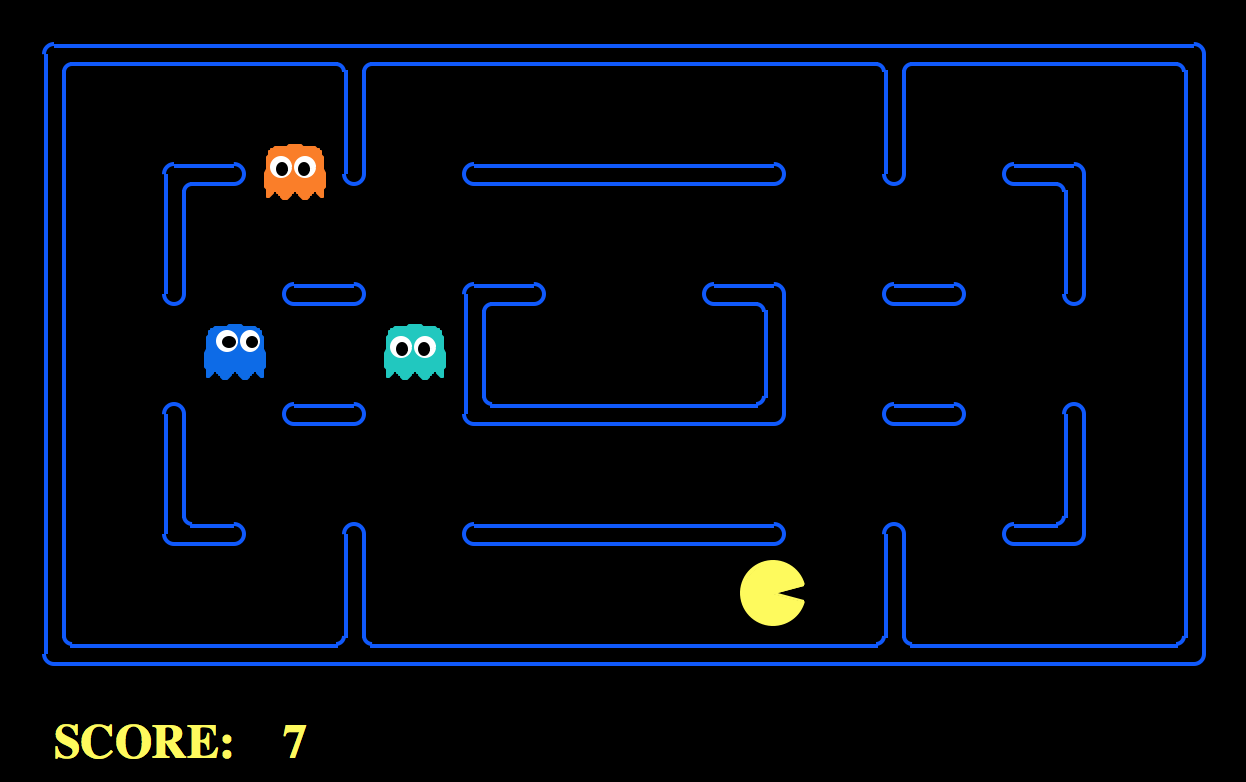
\includegraphics[width=\columnwidth]{examplemap.png}
	\caption{Game Play}
	\label{fig:gameplay}
\end{figure}

When we load in a map, we first convert it into a graph where each position (x, y coordinate) is only connected to positions that are reachable from it in one step (agents cannot go through walls). Once we have our graph, we precompute the shortest distances between any two positions in the map, using Floyd Warshall's cubic-runtime algorithm. These distances are stored and accessed in constant time by all agents at every step of the game. For example, in strategy 6, we simply make each ghost pick whatever action minimizes its distance to Pacman. For all of the other strategies, ghosts take distance into consideration, but there is also the added notion of trapping Pacman. We came up with a heuristic that successfully encourages ghosts to reduce the area that Pacman can maneuver in. Note that we introduce a bit of randomness in all algorithms just to account for different scenarios and generate more realistic simulations.

\subsection{Pacman Behavior}
It's important here to mention how Pacman behaves. We modeled Pacman as a Minimax Alpha-Beta pruning agent. At depth $d$, Pacman evaluates a particular state $s$ by the distance to the ghost closest to it. So Pacman tries to maximize this distance, while it assumes that ghosts actively try to minimize it. This is an accurate vision of the world but it is however lacking the knowledge that ghosts will try to trap it. This is because of two reasons. First, ghosts may not always be trying to trap Pacman (strategy 6 for example). Second, it's not realistic to assume that Pacman has a complete mental model of the other ghosts and is able to simulate the computations of all other ghosts before taking its action.

One more thing we should mention about Pacman is that in the case of strategy 4 in which Pacman overhears ghosts' communication, Pacman basically gains a depth of minimax for free because it knows exactly where the ghosts will be in one step. More importantly, Pacman's decision in this case is based on a more accurate model of the world, since Pacman no longer has to maximize a heuristic that does not take trapping into account, it can know exactly what the ghosts will do in the first step.

\subsection{First Setting}
\subsubsection{Trapping Heuristic}

\begin{figure}[H]
	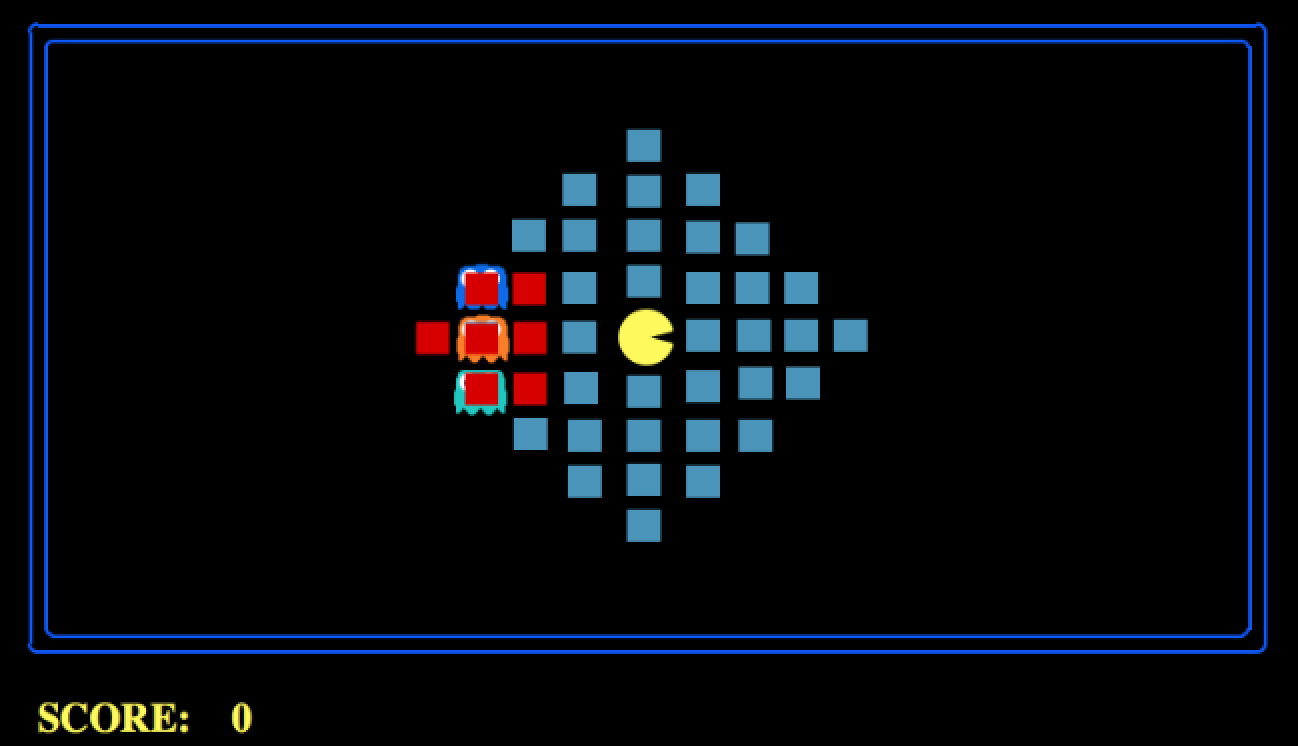
\includegraphics[width=\columnwidth]{badheuristic.png}
	\caption{Bad Heuristic}
	\label{fig:badheuristic}
\end{figure}

\begin{figure}[H]
	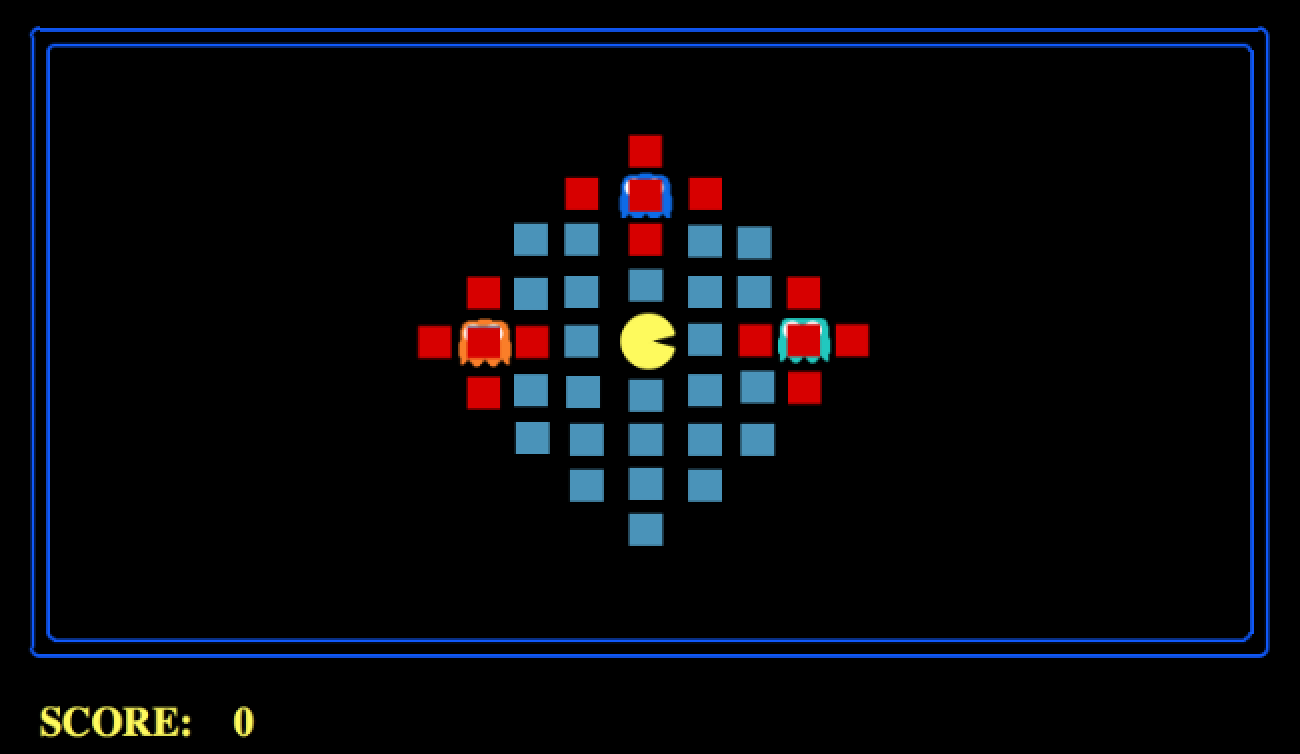
\includegraphics[width=\columnwidth]{goodheuristic.png}
	\caption{Good Heuristic}
	\label{fig:goodheuristic}
\end{figure}



This heuristic consists of two features. The first feature pertains to the distance between the ghost and Pacman. The second heuristic can be described as the total number of positions that are unsafe for pacman to be in, within a radius $r$. A position is unsafe if a ghost needs only one action to get there. To illustrate this, we can look at the following two images where the blue dots represent all the safe positions for Pacman within radius 4 and the red dots represent all the unsafe positions within radius 4. In figure \ref{fig:badheuristic}, the ghosts are close to each other so they only make seven dots unsafe. In figure \ref{fig:goodheuristic}, the ghosts are trapping pacman and they make 15 dots unsafe.\\ 

In the end, we settled on the following heuristic for each state $s$:
$$h(s) = u - 1.5d$$ Where $u$ is the number of unsafe positions in state $s$ within radius $r$, and $d$ is the distance to Pacman. This heuristic incentivizes both getting closer to Pacman (in order to minimize the distance and get within the radius $r$), as well as getting further away from each other.\\
To watch a short video demonstrating algorithms 6 and 1 in action with three ghosts, please visit the following url: \\
\url{www.youtube.com/watch?v=etU_Pud3HAM}



\subsubsection{Experiments}
We ran each algorithm for 100 games with 2, 3 and 4 ghost agents for each of two initial configurations. In the first initial configuration, all ghosts started off very close to each other in the top left corner of the map. In the second initial configuration, ghosts started off each at a corner of the map. The initial configurations are shown below for 4 ghosts

\begin{figure}[H]
	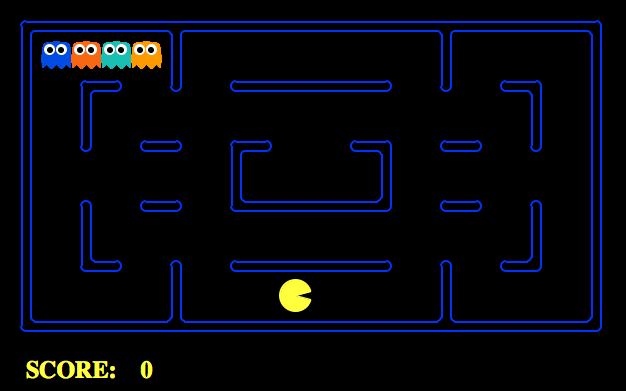
\includegraphics[width=\columnwidth]{maptogether.png}
	\caption{Map Together}
	\label{fig:maptogether}
\end{figure}

\begin{figure}[H]
	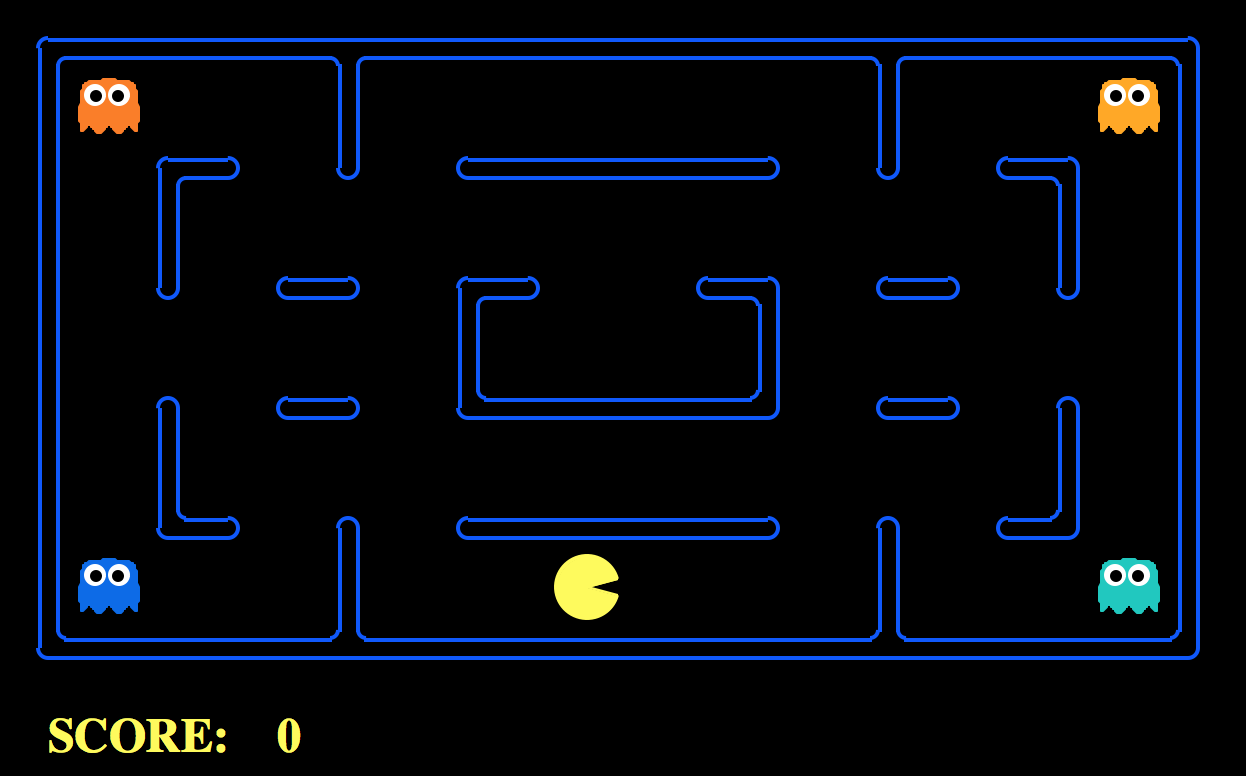
\includegraphics[width=\columnwidth]{mapcorners.png}
	\caption{Map Corners}
	\label{fig:mapcorners}
\end{figure}


\subsection{Second Setting}

\subsubsection{Framework Modifications}
When we load in a map, we not only precompute the shortest distances between any two positions in the map, but we precompute a sight grid which determines for every pair of positions if two agents can see each other (i.e. they are directly vertical or horizontal from each other and there is no wall between them) create a trail grid, which allows ghosts at a position to see how much trail has been left. Trail values max out at 250. Every time Pacman makes his turn, our system simulates trail decay by dividing all trail values by 1.25.  Finally, we modified the graphics of the framework to automatically display the value of the trail as a shade of red.

One issue with the sight modification is that it currently only works at the beginning on an agent's current turn. In the framework, agents takes turns to make actions.  If an action moves a Ghost into sight of Pacman, and Pacman moves out of sight on its immediate next turn, the ghost does not register sight of Pacman, since the sight check only occurs at the beginning of the Ghost's turn, not at the end.  This is surprisingly not easy to fix because of the probability system that ghosts use to make their next action and this case perceivable happens with frequency.

\subsubsection{Layouts}
\begin{figure}[H]
	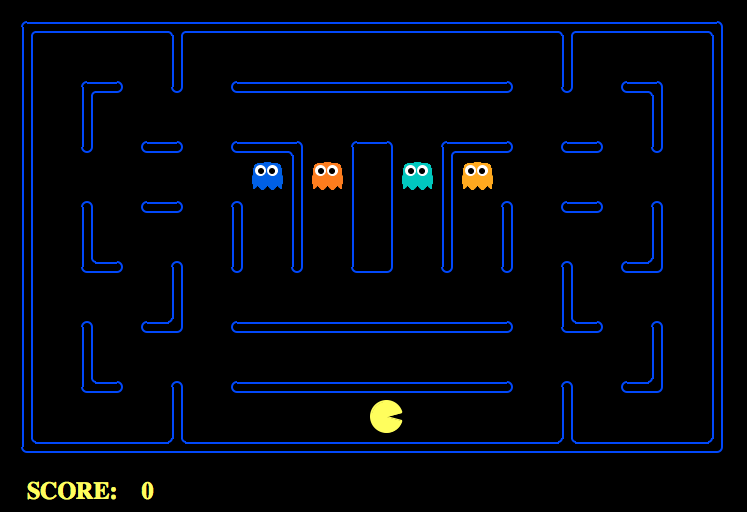
\includegraphics[width=\columnwidth]{StigmergyClassic1.png}
	\caption{Stigmergy Layout 1: Ghosts in Center}
	\label{fig:stigmap1}
\end{figure}
\begin{figure}[H]
	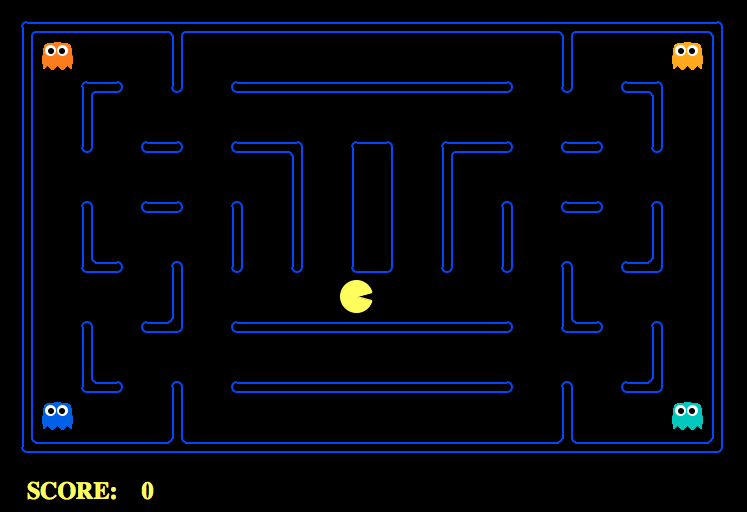
\includegraphics[width=\columnwidth]{StigmergyClassic2.png}
	\caption{Stigmergy Layout 1}
	\label{fig:stigmap2}
\end{figure}
For stigmergy, we modified the base medium classic layout from the Berkeley framework to be a big larger and to remove any 2x2 open spaces (so that everything consist of corridors or intersections).   

For this layout, we have two different starting locations for the ghosts and paceman.  One has the ghosts start in the center of the map with Pacman at the bottom (see figure \ref{fig:stigmap1}), and the other has ghosts start in the corners with paceman in the center (see figure \ref{fig:stigmap2}).  This is to help determine whether the starting position has an affect on our algorithms.




\subsubsection{Algorithms}

As our comparison algorithm, we implemented a BlindDirectionalGhost (see figure \ref{fig:blindghost}). A BlindDirectionalGhost acts randomly until it sights Pacman.  Upon sighting Pacman, it with high probability the shortest to Pacman's current position.  If BlindDirectionalGhost loses sight of Pacman, it keeps track of Pacman's last known position.  Upon arrive at the last known position, if BlindDirectionalGhost has not regained sight of Pacman, it clears it's knowledge of Pacman's position and acts randomly again.
\begin{figure}[H]
	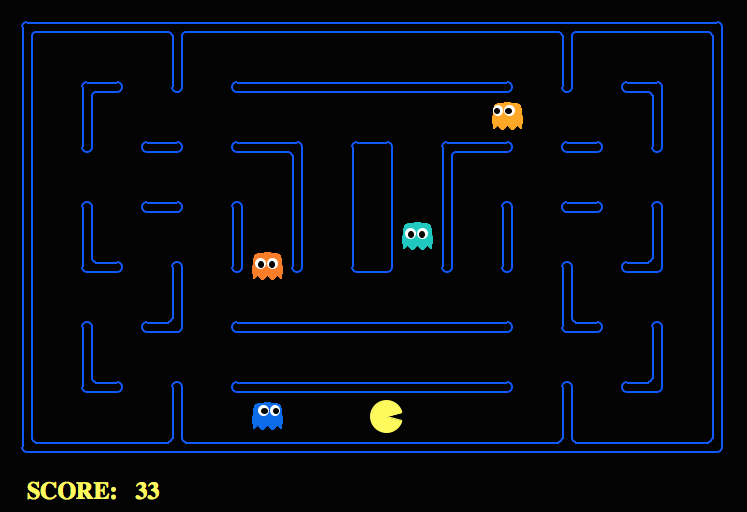
\includegraphics[width=\columnwidth]{BlindDirectionalGhost.png}
	\caption{BlindDirectionalGhost. Note the lack of trails.}
 	\protect\url{www.youtube.com/watch?v=dVFe-fwSLTs} 
	\label{fig:blindghost}
\end{figure}

For our RepulseStigmergyGhost  (see figure \ref{fig:repulseghost}), on seeing Pacman, our ghosts lay down the maximum trail of 250.  If they have an idea where Pacman is, they lay down a trail of (250 - trailvalue[currentpos]) / 2 (i.e. they decrease the difference between the maximum trail value and the current trail value by half).   If they have no idea where Pacman is, they automatically lay down a trail of (250 - trailvalue[currentpos]) / 4 (i.e. they decrease the difference between the maximum trail value and the current trail value by a quarter). In normal circumstances, RepulseDirectionalGhosts try to take the action that leads to the path with the least trail, with a probability of (sumOfSurroundingTrails - trailvalue[newpos])/(2 * sumOfSurroundingTrails). (excluding the special initial case of no trailvalues).

\begin{figure}[H]
	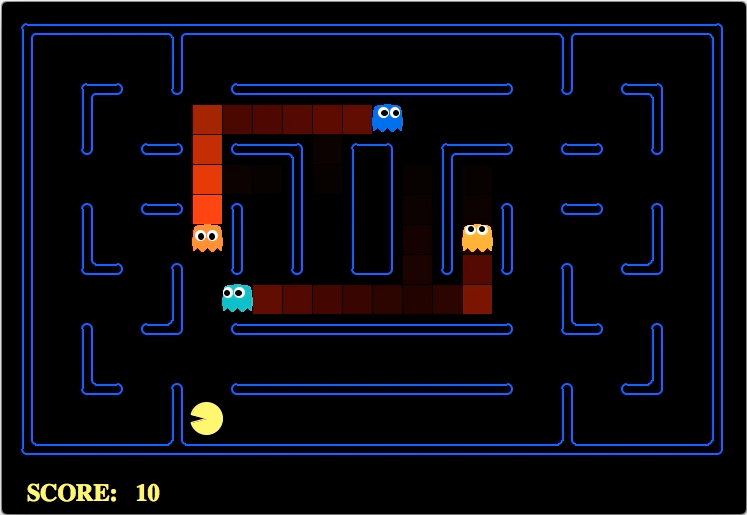
\includegraphics[width=\columnwidth]{RepulseGhost.png}
	\caption{RepulseStigmergyGhost. Note the creation of trails despite Pacman not being in sight at all.}
	\protect\url{www.youtube.com/watch?v=3o6VXkEG1uw} 
	\label{fig:repulseghost}
\end{figure}

For our AttractStigmergyGhost (see figure \ref{fig:attractghost}), on seeing Pacman, our ghosts lay down the maximum trail of 250.  If they have an idea where Pacman is, they lay down a trail of (250 - trailvalue[currentpos]) / 2 (i.e. they decrease the difference between the maximum trail value and the current trail value by half).   If they have no idea where Pacman is, they lay no trail at all. In normal circumstances, RepulseDirectionalGhosts try to take the action that leads to the path with the most trail, with a probability of (trailvalue[newpos])/(sumOfSurroundingTrails). (excluding the special initial case of no trailvalues).  

\begin{figure}[H]
	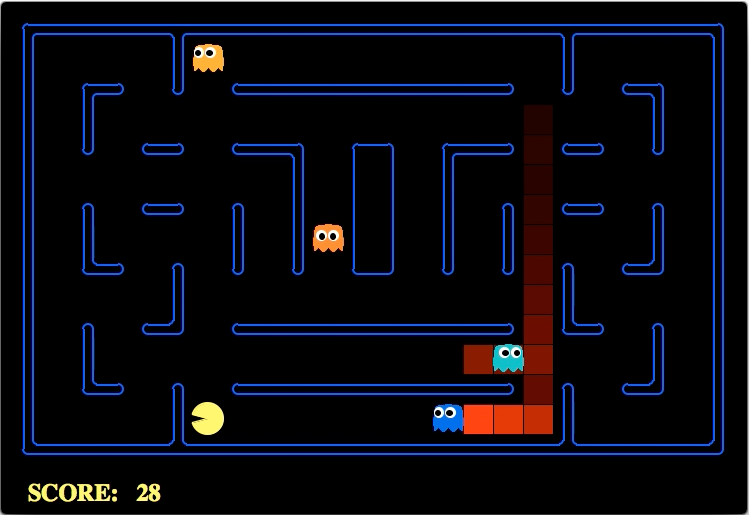
\includegraphics[width=\columnwidth]{AttractGhost.png}
	\caption{AttractStigmergyGhost. Note the creation of trails when Pacman is in sight but not when he isn't.}
	\protect\url{www.youtube.com/watch?v=qcaXzzpNs9s} 
	\label{fig:attractghost}
\end{figure}

For both stigmergy ghosts, we put a large penalty for taking an action that puts us in a shared position with another ghost, and we put a large weight on actions that make us closer to Pacman if he's in sight or closed to his last known position if we have one.

\subsubsection{Experiments}

For 2,3,and 4 ghosts on both layouts, we performed 50 trials each for both algorithms.  

For scoring our algorithms, the Berkeley framework has Pacman automatically gain a point every step it takes.  On ghost contact, Pacman loses 500 points.  Thus, we take the final score of every result and negate it in order to come up with a score for our algorithms.  We found early on that sometimes, the algorithms can run for an extremely long time because of the blind model, so we set a point of failure (when Pacman's score reaches 500).  Thus, each run gets a score from between 0 to 500, where 0 is when our algorithms fail (i.e. Pacman's score becomes 500, subtracted by the score loss from a ghost contact to keep scale), and 500 is Pacman being caught immediately (which is impossible).

\section{Results and Discussion}

\subsection{First Setting}
Now we will discuss our results from running the simulations described in the experimental setup. 

We first examine the amount of time it takes for an agent to compute an action under each algorithm. As Figure \ref{fig:averagecomputation} shows, the computation time to run algorithm 1 far exceeds the complexity of the other approaches. Algorithms 2 to four show relative similarities in complexity, which we certainly expect for algorithms 3 and 4; for algorithm 2 it is dependent on the team-size and in this setting with a team size of 2, we see a rough corespondence with algorithms 3 and 4. Algorithms 5 takes significantly less time than the other approaches, and algorithm 6 appears to take an almost negligible amount of time. 
\begin{figure}[H]
	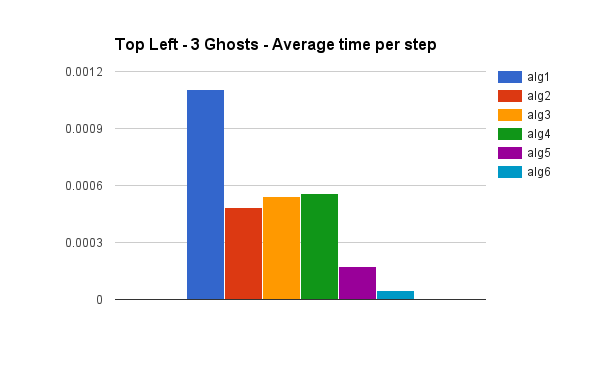
\includegraphics[scale=0.45]{time.png}
	\caption{Average Computation Time Per Step}
	\label{fig:averagecomputation}
\end{figure}	

We first examine the amount of time it takes for an agent to compute an action under each algorithm. As Figure \ref{fig:averagecomputation} shows, the computation time to run algorithm 1 far exceeds the computational time of the other approaches. This is in line with the theoretical asymptotic complexity of algorithm 1 which is $O(M^N)$ and exponentially slower than the other approaches. As expected, algorithms 3 and 4 take about the same time per step as well. In theory, algorithm 2 should take a longer time per step to run than algorithms 3 and 4 (its asymptotic runtime was exponentially larger), but for such small team sizes (a team of 1 and a team of 2), the exponent is dominated by the larger polynomial. Finally, as expected, algorithm 5 takes significantly less time than the other approaches, and algorithm 6 appears to take an almost negligible amount of time. 

\begin{figure}[H]
	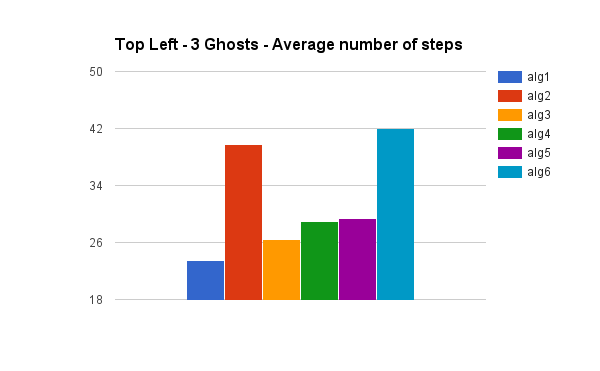
\includegraphics[scale=0.45]{leftsteps.png}
	\caption{Average Number of Steps from Top Left}
	\label{fig:averagenumstepsleft}
\end{figure}

\begin{figure}[H]
	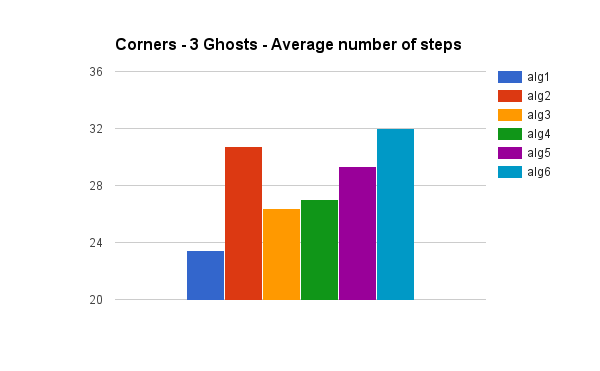
\includegraphics[scale=0.45]{cornersteps.png}
	\caption{Average Number of Steps from Corner}
	\label{fig:averagenumstepscorner}
\end{figure}

\noindent We next want to explore the number of steps it takes for ghosts to capture Pacman according to the algorithm they follow under each of our initializations. In this case, the fewer steps it takes to capture Pacman, the better our performance is. Before we start discussing our results, our intuition tells us that algorithm 1 should perform best because every possible combination of actions is evaluated and if our heuristic is a good proxy for capturing Pacman, then there is no scenario where algorithm 1 is consistently beaten by another algorithm. Similarly, we would expect algorithm 2 to perform well but not as well as algorithm 1. It's not clear a priori whether algorithm 2 performs better than algorithm 3 or not. It's also not clear that algorithm 3 performs better than algorithm 4 although we would expect it to as long as Pacman's overhearing causes it to take smarter actions. We would also expect algorithm 3 to perform better than algorithm 5 because the heuristics would be evaluated based on more accurate states of the world that are guaranteed by other ghosts through communication. Finally, we would expect algorithm 6 to perform the worst between all algorithms because there is no explicit trapping behavior and it is theoretically possible that ghosts can chase Pacman Ad Infinitum (it it wasn't for a slight element of randomness that we incorporated in our action decision). \\
Looking at the results in Figure 9 and 10, we notice that in both initial configurations, algorithm 1 takes the fewest amount of steps, and algorithm 6 takes the largest amount of steps (as we had expected). However, Figure \ref{fig:averagenumstepsleft} and Figure \ref{fig:averagenumstepscorner} reveal that surprisingly algorithm 2 takes a much higher amount of steps to capture Pacman than the other approaches except algorithm 6 (all of which seem to scale in inverse order of their complexity). We can explain this by noting that each subteam in algorithm 2 does not even take into account the positions of other ghosts outside of the subteam. This turns out to drastically affect the success rate because even in the case of algorithm 5 where agents do not explicitly collaborate, there is at least an implicit coordination between their actions even if that coordination is not entirely accurate.\\
We also notice that algorithm 4 seems to consistently behave slightly worse than algorithm 3, so Pacman's overhearing does actually allow to take smarter decisions to counter the coordination of ghost agents. The difference in performance is not large enough to make algorithm 5 more successful than algorithm 4 so there is still some value in unencrypted communication so long as the $S$ cost mentioned earlier is high enough to warrant the dip in the success rate between algorithms 3 and 4.\\
A very important observation we can make by comparing these two figures is that while the ordering of the algorithms is the same for both initial configurations, we notice that the spread between the algorithms is greatly reduced when the ghosts start at different corners. In fact, the difference between algorithms 1 and 6 when all ghosts start at top left is 18.5 steps on average, whereas it is only 8.6 on average when the ghosts start at different corners. The same pattern follows for all other algorithms, they all perform better in the corners initialization configuration, but the differences between the algorithms is greatly reduced for the corners initialization. For the corners configuration in particular, we can interpret this finding by observing the actual games and noticing that Pacman (who tries to minimize the distance to the closest ghost) has no preferred direction to take since ghosts are coming from all directions, so in a way, Pacman is already trapped even without any explicit trapping heuristics built into the ghost agents. From this observation, we conclude that depending on the initial configuration, the additional benefit from employing a more complex algorithm might not be worth the added time complexity anymore.\\\\

We transition now to examining our aggregated results collected for each of 2, 3, and 4 ghosts, presented in the tables in Figures 11, 12 and 13. 

\end{multicols}

\begin{figure}[H]
	\centering{
	\includegraphics[width=0.85\textwidth]{timeValgs.png}
	}
	\caption{Number of Seconds to Generate Each Action}
\end{figure}

\begin{figure}[H]
	\centering{
	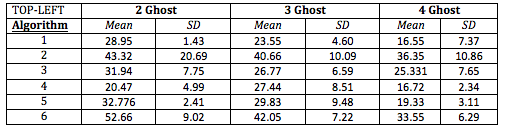
\includegraphics[width=0.85\textwidth]{TopLeftScore.png}
	}
	\caption{Number of Steps till Capture for Top Left Initilization}
\end{figure}

\begin{figure}[H]
	\centering{
	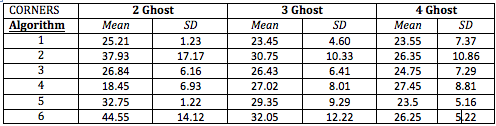
\includegraphics[width=0.85\textwidth]{CornersScore.png}
	}
	\caption{Number of Steps till Capture for Corners Initilization}
\end{figure}


\begin{multicols}{2}

From Figure 11, we notice that the average time per step is constant for algorithm 6 regardless of the number of ghosts. For all other algorithms, the average time per step grows with the number of ghosts at rates corresponding with our predictions through the runtime complexity of each algorithm.\\
From Figures 12 and 13, we notice that as noted before, the spread between algorithms decreases when the ghosts are initially at different corners (for all values of the number of ghosts). Interestingly, we also notice that all algorithms seem to perform better when the number of ghosts increases, and the spread between algorithms (from best to worst) seems to also decrease as the number of ghosts increases. This is particularly significant because it means that as the number of ghosts increases, a distributed algorithm like algorithm 5 becomes closer and closer in performance to algorithm 1. Couple that finding with the fact that centralized systems becomes much less scalable and tractable for larger values of $N$, and we conclude that it's always better to pick a distributed algorithm like algorithm 5 as the number of predators increases.

Finally, we are interested in assessing the accuracy of our heuristic as a proxy for likelihood of capture success. We compare the progression of heuristic values in a game for each of the algorithms from 1 to 5. Note that we ignore algorithm 6 because there is no heuristic component to it.\\
\begin{figure}[H]
	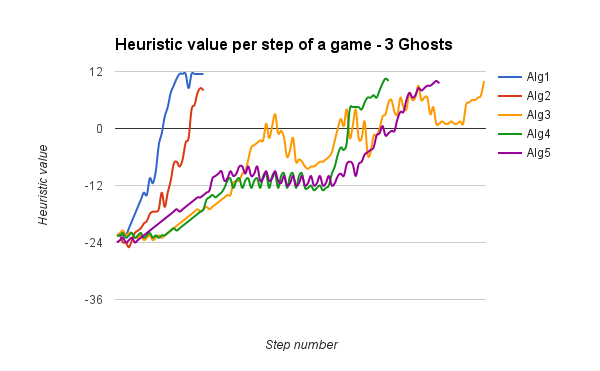
\includegraphics[scale=0.45]{heuristicvalues.png}
	\caption{Heuristic value progression per algorithm}
\end{figure}

\noindent In Figure 14, we notice that the lines end when a heuristic value of close to 12 is reached. This indicates that the game has ended because the capture was successful, so the heuristic value is consistent and accurate when the ghosts are about to capture Pacman. We also notice that the lines are monotonically increasing for the most part (this is not as clear for algorithm 3 but it is probably particular to that specific game perhaps because of the randomness that we introduced into the decision making). This means that the heuristic value is successfully guiding the agents towards success. These two observations lead us to conclude that our heuristic very accurately measures the predators' improvement toward capturing the prey. 

\subsection{Second Setting}

For our stigmergy tests, we recorded the scores and calculated the averages and number of failures for each algorithm and for each ghost. 

Examining figure \ref{fig:stigmergystats1} and figure \ref{fig:stigmergystats2} reveal that both stigmergy algorithms perform significantly better than the BlindDirectionalGhost.  Furthermore, the success of the Stigmergy algorithms seem to scale rapidly with the number of ghosts: 4 ghosts are sufficient to prevent failure to capture Pacman, and average scores for both layouts near or exceed 400 with 4 ghosts. 

Layouts had a small effect on the stigmergy algorithms, in particular, both algorithms perform appreciably better on layout 2 with 3 ghosts.  However, BlindDirectionalGhost does extremely poorly with 2 ghosts on layout 2, failing every time.  All together, the two layouts did not determine overall efficacy.

Examining figures \ref{fig:stigmergyresultslayout1} and \ref{fig:stigmergyresultslayout2} tell similar stories.  BlindDirectionalGhost does poorly with any number of ghosts.  Both Repulse and Attract Stigmergy agents score improve with the number of ghosts both in average score but also in number of failures and in consistency (smaller standard deviations).

\end{multicols}
\begin{figure}[H]
	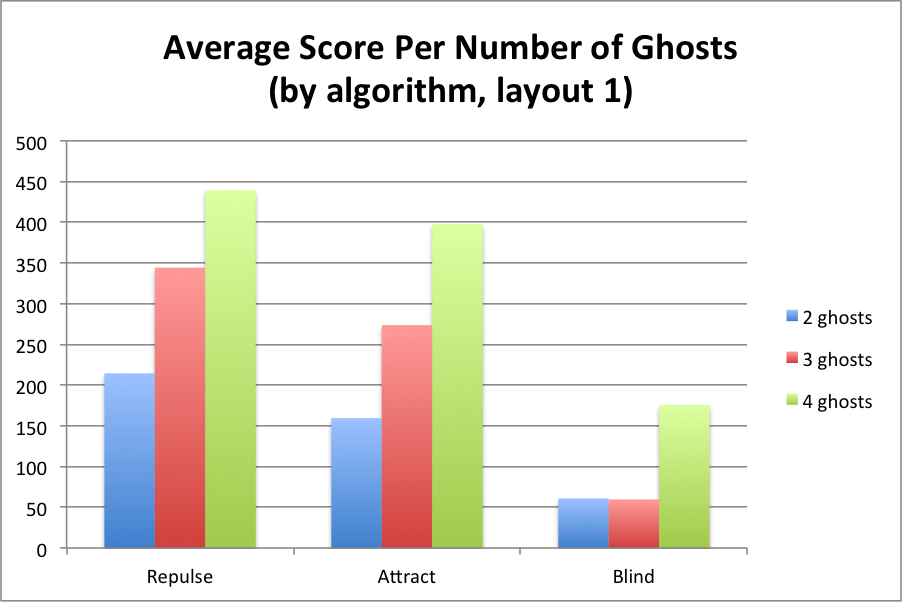
\includegraphics[width=0.5 \columnwidth]{stigmergytrendclassicscore.png}
	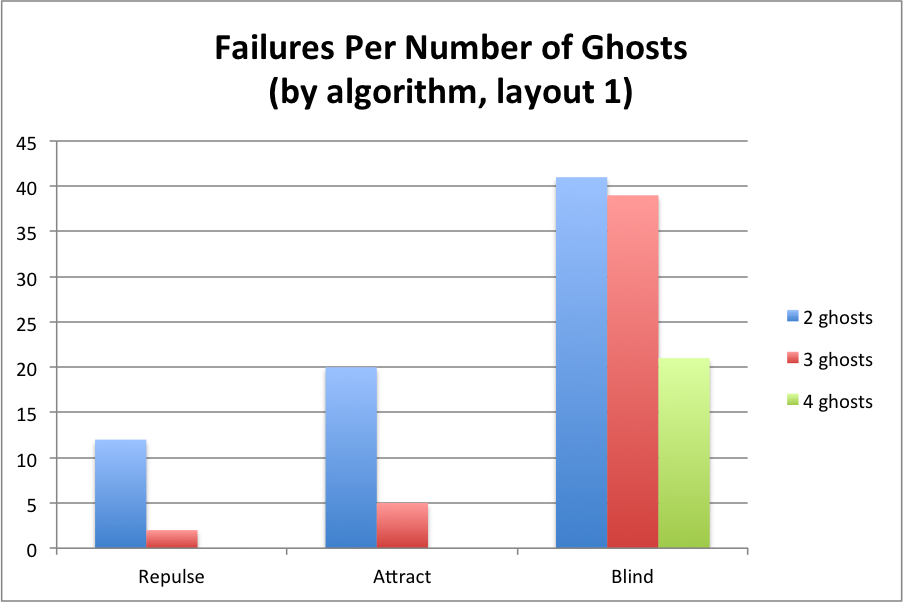
\includegraphics[width= 0.5 \columnwidth]{stigmergytrendclassicfail.png}
	\caption{Average Score and Number of Failures for Stigmergy Layout 1.  A larger average score and a low number of failures is better.}
	\label{fig:stigmergystats1}
\end{figure}

\begin{figure}[H]
	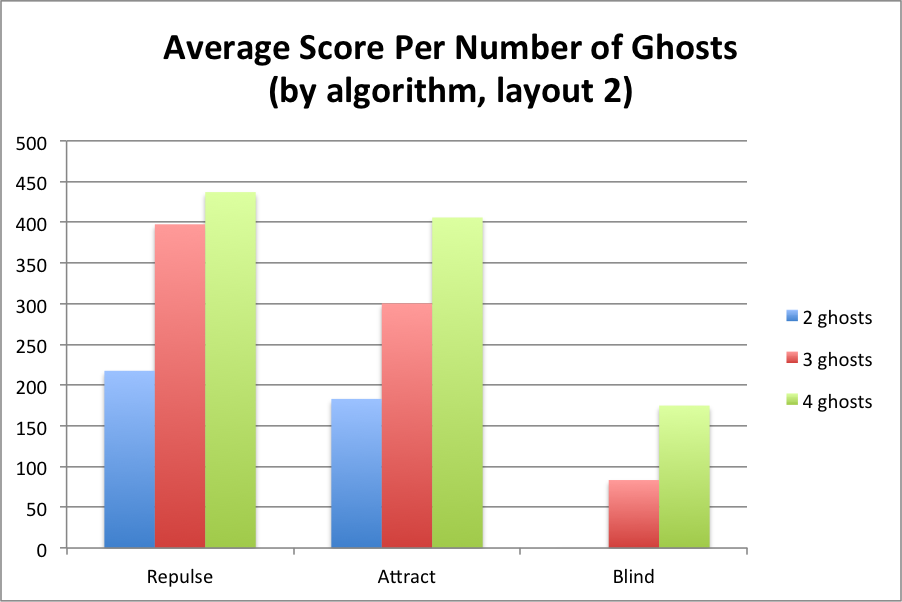
\includegraphics[width=0.5 \columnwidth]{stigmergytrendaltscore.png}
	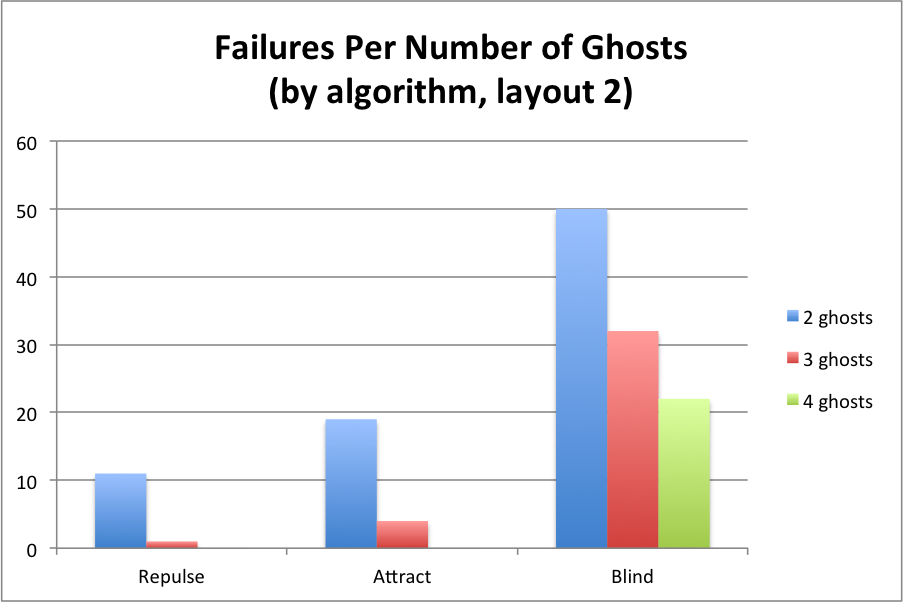
\includegraphics[width= 0.5 \columnwidth]{stigmergytrendaltfail.png}
	\caption{Average Score and Number of Failures for Stigmergy Layout 2. A larger average score and a low number of failures is better.}
	\label{fig:stigmergystats2}
\end{figure}

\pagebreak
\begin{figure}[H]
	\centering{
	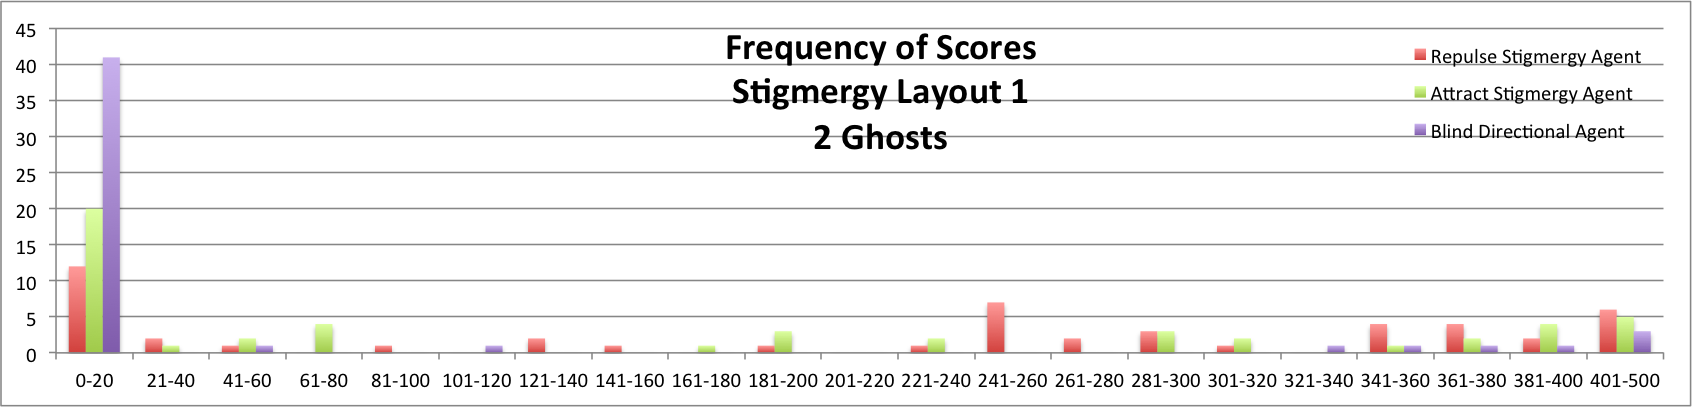
\includegraphics[width=\textwidth]{stigmergyresultsclassic2.png}
	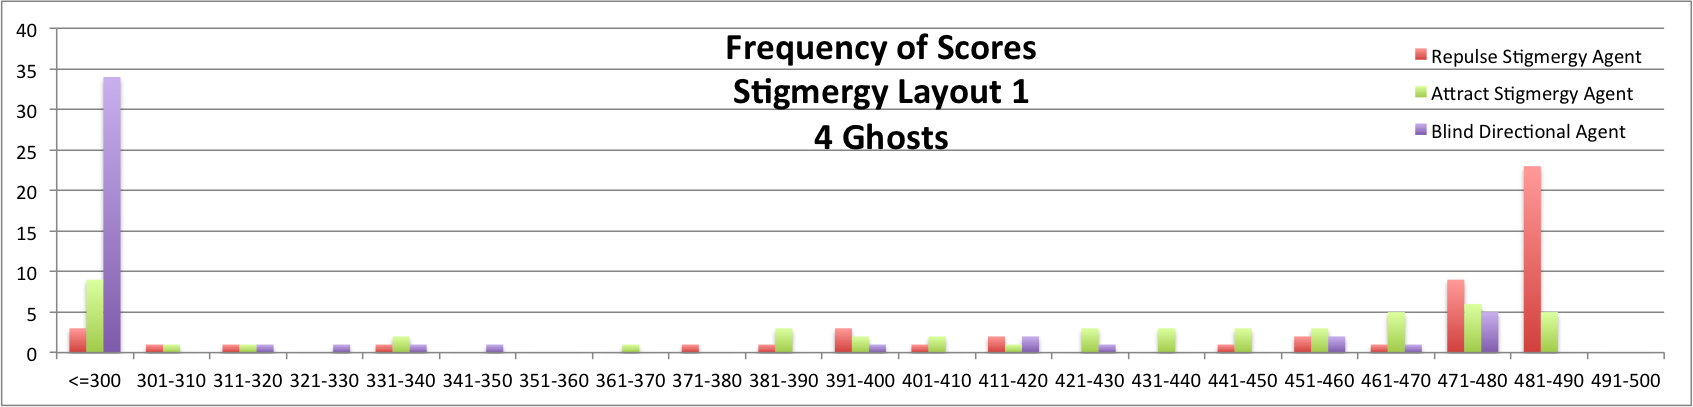
\includegraphics[width=\textwidth]{stigmergyresultsclassic4.png}
	\caption{Histograms showing the frequency distribution of ghost scores for each agent (higher scores are better) for Layout 1, with 2 and 4 ghost agents. Average Scores for 2 Ghosts (repulse, attract, blind): 214.4, 159.46, 60.82; 4 Ghosts: 439.34, 397.78, 175.62; Standard Deviations for 2 Ghosts: 158.45,170.85, 145.78; 4 Ghosts: 78.79, 88.88, 188.80}
	\label{fig:stigmergyresultslayout1}
	}
\end{figure}

\begin{figure}[H]
	\centering{
	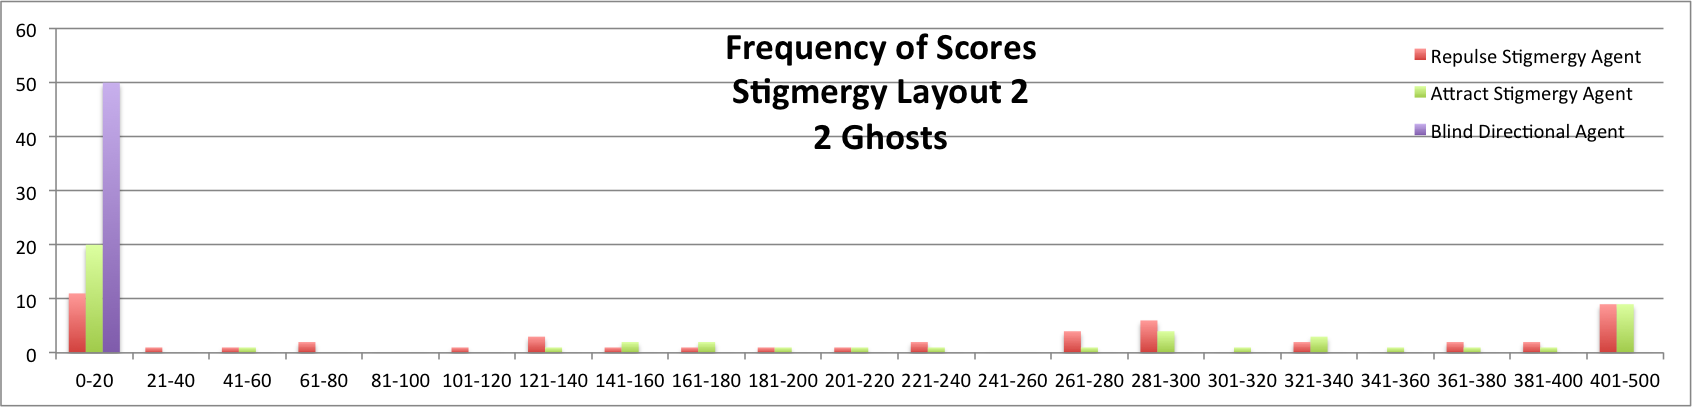
\includegraphics[width=\textwidth]{stigmergyresultsalt2.png}
	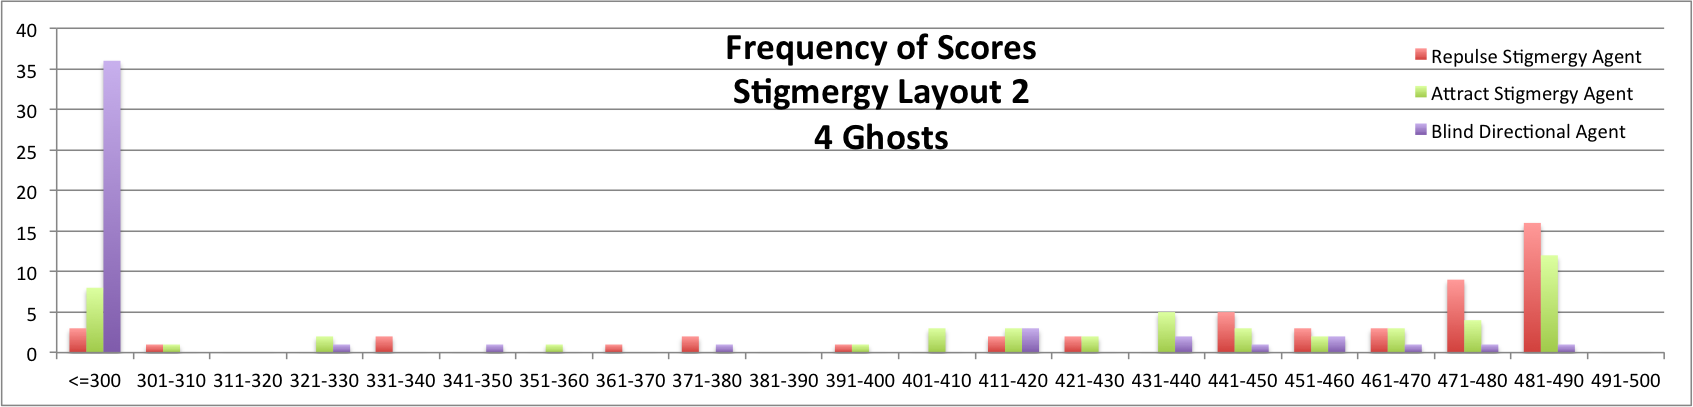
\includegraphics[width=\textwidth]{stigmergyresultsalt4.png}
	\caption{Histograms showing the frequency distribution of ghost scores for each agent (higher scores are better) for Layout 2, with 2 and 4 ghost agents. Average Scores for 2 Ghosts (repulse, attract, blind): 217.64, 183.12, 0; 4 Ghosts: 437.04, 405.86, 174.92; Standard Deviations for 2 Ghosts: 162.9668503, 173.4814746, 0; 4 Ghosts: 73.54, 101.35,187.04}
	\label{fig:stigmergyresultslayout2}
	}
\end{figure}
\pagebreak
\begin{multicols}{2}

\section{Conclusion}
We present six different algorithms with varying degrees of collaborative complexity that can be employed by a pack of predators in a predator/prey multi-agent system. By modeling the system as a Pacman vs Ghosts game and simulating runs for each of our algorithms, we have reached the following main conclusions: 1- The algorithms generally succeed proportionally to their complexity. 2- The difference between the success of the algorithms is greatly reduced in a starting configuration where predators are scattered as opposed to one in which they are close to each other. 3- The difference between the success of the algorithms is reduced when the number of predators increases. As a result, a large pack of predators should employ distributed algorithms because their tractability greatly outweighs their performance deficiencies. 4- The heuristic that we present for trapping a prey is very accurate.

Furthermore, we demonstrate that our two stigmergy algorithms are significantly better than our BlindDirectionalGhost benchmark.  RepulseStigmergyGhost performs overall better than AttractStigmergyGhosts, but both scale well with the number of ghosts, scoring higher and becoming more consistent, and, with the limited testing we did, are somewhat layout independent.  Both are also robust enough to prevent failure to capture Pacman with 4 ghosts.

\section{Future Directions}
The work we conducted in this project and some of the results we observed have inspired us to think of future directions we would like to take this research, given additional time.

As discussed earlier, we were initially surprised to see how poorly algorithm 2, where we break up our agents into sub-teams, performed relative to the other approaches and our expectations. When trying to reason through why this may be the case, we realized that all the ghosts in a particular sub-team do not acknowledge in any manner the ghost agents in the other sub-teams and are ignorant of even their positions, let alone their intentions. In a future work, we would like to test a few different adaptions of this approach. In the first approach, agents in a sub-team would be able to see ghost agents in another sub-team and not explicitly communicate with them, but would attempt to reason where they might go (similar to what individual agents do in algorithm 5). In a different approach, we would allow the subteams to communicate with each other. This follows work from Roth et al. where individual agents decide whether to communicate with one another based on whether they believe it will change the joint-action taken by the team; similarly, in this case sub-teams will choose to communicate with one another or not based on whether the sub-team believes it will change the joint action of all the ghost agents.

Another potential future direction of this project that we are very excited about involves coming up with a hybrid algorithm that has all six of our collaboration algorithms in its arsenal and decides on which one to apply based on the state of the game. The motivation behind this approach is the realization that collaboration and trapping behavior have very different benefits depending on the state of the game and the relative positions of the agents. For example, if all the ghost agents are very far away from Pacman, then it may not be worth the computational cost to use full communication approaches like algorithm 1, and instead the agents should simply try to get closer to Pacman like in algorithm 6. However, when the ghost agents are close enough to actually employ trapping behavior, then we may want to switch our approach to allow full communication, as the computational complexity may now be justified in light of potentially optimized performance. We believe that future work that tries to devise an algorithm, perhaps through reinforcement learning, that decides which approach to use based on the state of the game would be extremely interesting and useful.

For the stigmergy approaches, it would be interesting to combine additional communication methods to see how effective a joint system would be.  Additional testing on more layouts and testing scaling beyond 4 ghosts would also be interesting directions.

\section{Division of Work}
Sami and Devvret worked together on setting 1 and all of its related components. Sami implemented the graph conversion and the pre-computation of distances as well as both modes of Pacman (regular Alpha Beta pruning agent and Overhearing minimax agent in the case of algorithm 4). Dev focused on modifying the game framework to allow for each of our six scenarios. Sami and Dev implemented algorithms 5 and 6 together, as they were the first approaches implemented and benefited from early collaboration and discussion. After that, Sami led the effort for the implementations of algorithms 1 and 4 and Dev led the effort for the implementations of algorithms 2 and 3. Both Sami and Dev worked together to test different ideas for heuristics, and derived the heuristic currently in use and tested its rigor across the different algorithms. When conducting the simulations to generate our results, Dev worked more so on data collection and parsing, while Sami worked on data analysis and visualization.  

George worked exclusively on setting 2, and all algorithms developed and results generated related to stigmergy were a result of his efforts.

\bibliographystyle{plain}
\bibliography{bibliography.bib}


\end{multicols}

\end{document}
